%%%%%%%%%%%%%%%%%%%%%%%%%%%%%%%%%%%%%%%%%%%%%%%%%%%%%%%%%%%%%%%%%%%%%%%%%%%%% 
%
% This is a LaTeX file for an A0 poster.
% 
% template poster taken from https://canizo.org/latex_poster
%
%%%%%%%%%%%%%%%%%%%%%%%%%%%%%%%%%%%%%%%%%%%%%%%%%%%%%%%%%%%%%%%%%%%%%%%%%%%%% 

%%%%%%%%%%%%%%%%%%%%%%%%%%%%%%%%%%%%%%%%%%%%%%%%%%%%%%%%%%%%%%%%%%%%%%%%%%%%% 
%%%%%%%%%%%%%%%%%%%%%%%%%%%%%%%%%%%%%%%%%%%%%%%%%%%%%%%%%%%%%%%%%%%%%%%%%%%%%
%
% Towards a standardized workflow for mass spectrometry based single-cell 
% proteomics
%
% Poster for the Applied Bioinformatics for Life Science, February 2020, Leuven.
%
%%%%%%%%%%%%%%%%%%%%%%%%%%%%%%%%%%%%%%%%%%%%%%%%%%%%%%%%%%%%%%%%%%%%%%%%%%%%%
%%%%%%%%%%%%%%%%%%%%%%%%%%%%%%%%%%%%%%%%%%%%%%%%%%%%%%%%%%%%%%%%%%%%%%%%%%%%%

\documentclass{article}
% To modify the size of the page:
\usepackage[dvips,a3paper,portrait,centering,margin=0.5cm]{geometry}
% To create multiple columns
\usepackage{multicol}

\usepackage[utf8]{inputenc}
% To align images
\usepackage[export]{adjustbox}
% Use captions in minipages
\usepackage{caption}
% Math font
\usepackage{amsmath, amsthm, amsfonts}
% Include figure files.
\usepackage{graphicx}

% Coding fonts
% ------------
% For including R chunks 
\usepackage{listings} 
\lstset{
  language=R,
  basicstyle=\small\ttfamily\color{vdgray},       % the size of the fonts that are used for the code
  % sensitive=false,
  numbers=left,                   % where to put the line-numbers
  numberstyle=\tiny\color{gray},  % the style that is used for the line-numbers
  stepnumber=1,                   % the step between two line-numbers.
  numbersep=0.1cm,                % how far the line-numbers are from the code
  backgroundcolor=\color{lgray},  % choose the background color. You must add \usepackage{color}
  deletekeywords={stat},
  keywordstyle=\color{blue},      % keyword style
  stringstyle=\color{green},      % string literal style
  xleftmargin=0.5cm,
}
% Create command for highlighting inline code or variables
\newcommand{\hcode}[2][lgray]{{\ttfamily\color{vdgray}\colorbox{#1}{#2}}}

% Colors
% ------
\usepackage{color}
\usepackage[dvipsnames]{xcolor}
% Color panel used throughout the poster
\definecolor{lgray}{rgb}{0.9179688,0.9179688,0.9179688} % #ebebeb
\definecolor{dgray}{rgb}{0.796875,0.796875,0.796875} % #cccccc
\definecolor{vdgray}{rgb}{0.3984375,0.3984375,0.3984375} % #666666
\definecolor{coral}{rgb}{0.9960938,0.4960938,0.3125000} % #ff7f50
\definecolor{blue}{rgb}{0.4218750,0.6484375,0.8007812} % #6ca6cd
\definecolor{green}{rgb}{0.6992188,0.7265625,0.5078125} % #b3ba82
\definecolor{yellow}{rgb}{0.9570312,0.8671875,0.6992188} % #f5deb3

% Adjust space between reference items
% ------------------------------------
\let\OLDthebibliography\thebibliography
\renewcommand\thebibliography[1]{
  \OLDthebibliography{#1}
  \setlength{\parskip}{0pt}
  \setlength{\itemsep}{0pt plus 0.3ex}
}
  
\pagestyle{empty}

\def\to{\rightarrow}


% ===========================================================================

\title{}
\author{}
\date{}

\begin{document}


% ---------------------------------------------------------------------------
% Banner


\begin{center}
\colorbox{lgray}{
  \begin{minipage}{3.7cm}
    \includegraphics[width=1.2\linewidth]{figs/DSC_2812.jpg}
  \end{minipage}
  %&
  \begin{minipage}{.72\textwidth}
    \begin{center}
      % Title 
      \vspace{0.4cm}
      \huge 
      \hspace{1cm}
      \noindent
      \textbf{Towards a standardized workflow for mass spectrometry based single-cell proteomics} \\
      \vspace{0.4cm}
      % Authors
      \Large \textbf{Christophe Vanderaa, Laurent Gatto} \\
      % Affiliation
      \Large \textit{Computational biology and bioinformatics, de Duve Institute, UCLouvain } \\
      % email
      \vspace{0.4cm}
      \normalsize christophe.vanderaa@uclouvain.be \\
      \hspace{1cm}
    \end{center}
  \end{minipage}
  %&
  \begin{minipage}{3.7cm}
      
\includegraphics[width=0.7\linewidth, right]{figs/fnrs.png} \\
      \vspace{0.5cm}
      
\includegraphics[width=1.1\linewidth, right]{figs/ucl.png}
  \end{minipage}
}
\end{center}


% ---------------------------------------------------------------------------
% Summary + conclusion
\noindent
% Summary
\colorbox{yellow}{
  \noindent
  \begin{minipage}[t]{13.7cm}
  \vspace{.15cm}
    \section*{\huge Summary}
    \large 
    Recent advances in sample preparation, processing and mass spectrometry (MS) have allowed the emergence of MS-based \textbf{single-cell proteomics} (SCP). In order to boost the development of SCP methodologies, we are developing a suite of packages that contain curated data sets (\textbf{\hcode[yellow]{scpdata}}) and dedicated functions (\textbf{\hcode[yellow]{scp}}). It relies on a standardized data structure combining Bioconductor classes used for singe cell analyses (\textbf{\hcode[yellow]{SingleCellExperiment}}), and MS-based proteomics analyses (\textbf{\hcode[yellow]{Features}}) facilitating re-use of current state-of-the-art methodologies.
    \vspace{0.1cm}
  \end{minipage}
}
\hspace{0.37cm}
% Conclusion
\noindent
\colorbox{yellow}{
  \begin{minipage}[t]{13.6cm}
    \vspace{.2cm}
    \section*{\huge Conclusion}
    \vspace{0.35cm}
    \large
    MS-based SCP is still in its infancy. Nevertheless, the \hcode[yellow]{scpdata} experiment package offers a growing repository of curated data ideally suited for \textbf{method benchmarking} and \textbf{data QC}. This will enable us to develop new methodologies to tackle the current hurdles that MS-SCP faces: missing data, batch effect, and high dimensionality. 
    \vspace{0.57cm}
 \end{minipage}
}
\vspace{-1cm}


% ---------------------------------------------------------------------------
% Create a 2 column layout
\setlength{\columnsep}{0.5cm}
\begin{multicols}{2}

% ---------------------------------------------------------------------------
% Introduction
\noindent
\begin{minipage}[t]{\linewidth}
  \vspace{0.5cm}
  \section*{\huge Introduction}
  \large
  There are two main pipelines able to generate MS-SCP data:
  \textbf{\large nanoPOTS pipeline} (Zhu et al., 2018, \cite{Zhu2018-bf}) runs label-free proteomics for single cells. The \textbf{\color{BrickRed}{throughput is low}} ($\pm$ 10 samples/day), but it achieves \textbf{\color{OliveGreen}{accurate peptide quantification}}. 
    \vspace{-0.3cm}
    \begin{center}
      
\includegraphics[width=0.87\linewidth]{figs/nanopots.png} \\
    \end{center}
    \vspace{-0.3cm}
  \textbf{\large SCoPE pipeline} (Budnik et al., 2018, \cite{Budnik2018-qh}) adapts TMT-based proteomics to single-cells. The \textbf{\color{OliveGreen}{throughput is higher}} ($\pm$ 5 samples/hour), but it suffers from \textbf{\color{BrickRed}{presence of chemical noise}}.
    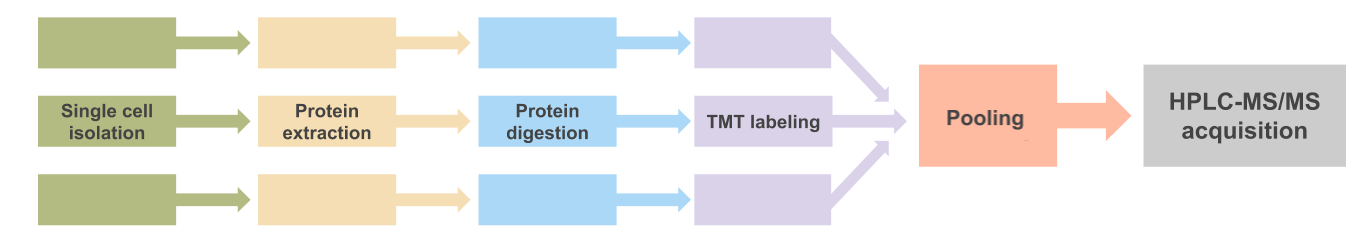
\includegraphics[width=0.9\linewidth]{figs/scopems.png} \\
    \vspace{-0.3cm}
\end{minipage}


% ---------------------------------------------------------------------------
% Data manipulation
\noindent
\begin{minipage}[t]{\linewidth}
  \vspace{0.55cm}
  \section*{\huge Data manipulation}
  \large
  The Bioconductor class \hcode{MSnSet} is a reliable framework for \textbf{standard and systematic} quantitative data processing. Below, we have reproduced the analysis pipeline from \cite{Specht2019-jm}:
  \begin{lstlisting}
    data("specht2019_peptide")
    specht2019_peptide %>% 
      scp_normalize_stat(what = "row", mean, "-") %>%
      scp_aggregateByProtein() %>%
      scp_normalize_stat(what = "column", median, "-") %>%
      scp_normalize_stat(what = "row", mean, "-") %>%
      imputeKNN(k = 3) %>%
      batchCorrect(batch = "raw.file", target = "celltype") -> scpd
  \end{lstlisting}
\end{minipage}


% ---------------------------------------------------------------------------
% Data visualization
\noindent
\begin{minipage}[t]{\linewidth}
  \vspace{0.5cm}
  \section*{\huge Data visualization}
  \large
  \hcode{scpdata} also offers an ideal environment for benchmarking. It will contain a wide variety of MS-SCP data sets from \textbf{well-defined synthetic standards} to \textbf{real biological samples}. Different methods can be compared using \textbf{objective benchmarking metrics} or \textbf{visualization} with dimension reduction (Figure \ref{fig:pca}).
  \begin{center}
    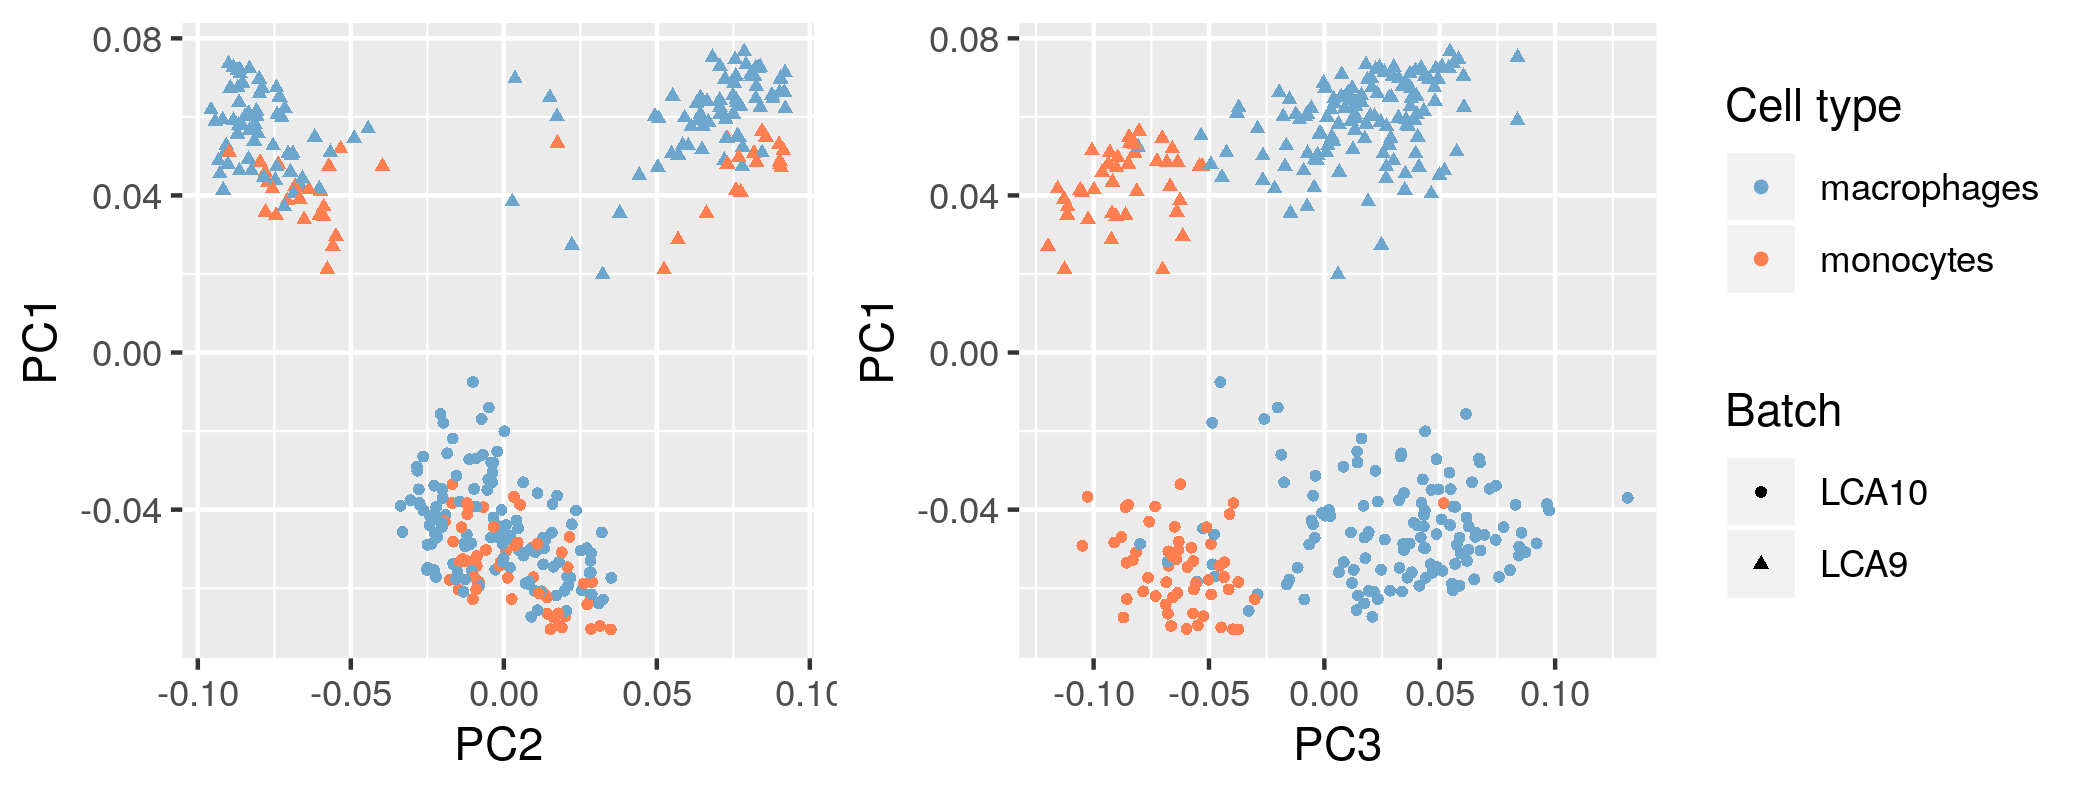
\includegraphics[width=\textwidth]{figs/PCA.png}
  \end{center}
  \captionof{figure}{\textbf{PCA plot of peptide expression data.} \small Macrophages and monocytes are well separated in the third principal component. However, the first and second components are driven by batch effects. LCA10 and LCA9 are two chromatographic batches. The PCA was performed using the NIPALS algorithm.}
  \label{fig:pca}

\end{minipage}

% ---------------------------------------------------------------------------
% Data structure
\noindent
\begin{minipage}[t]{\linewidth}
  \vspace{0.55cm}
  \section*{\huge Data Structure}
  \begin{center}
    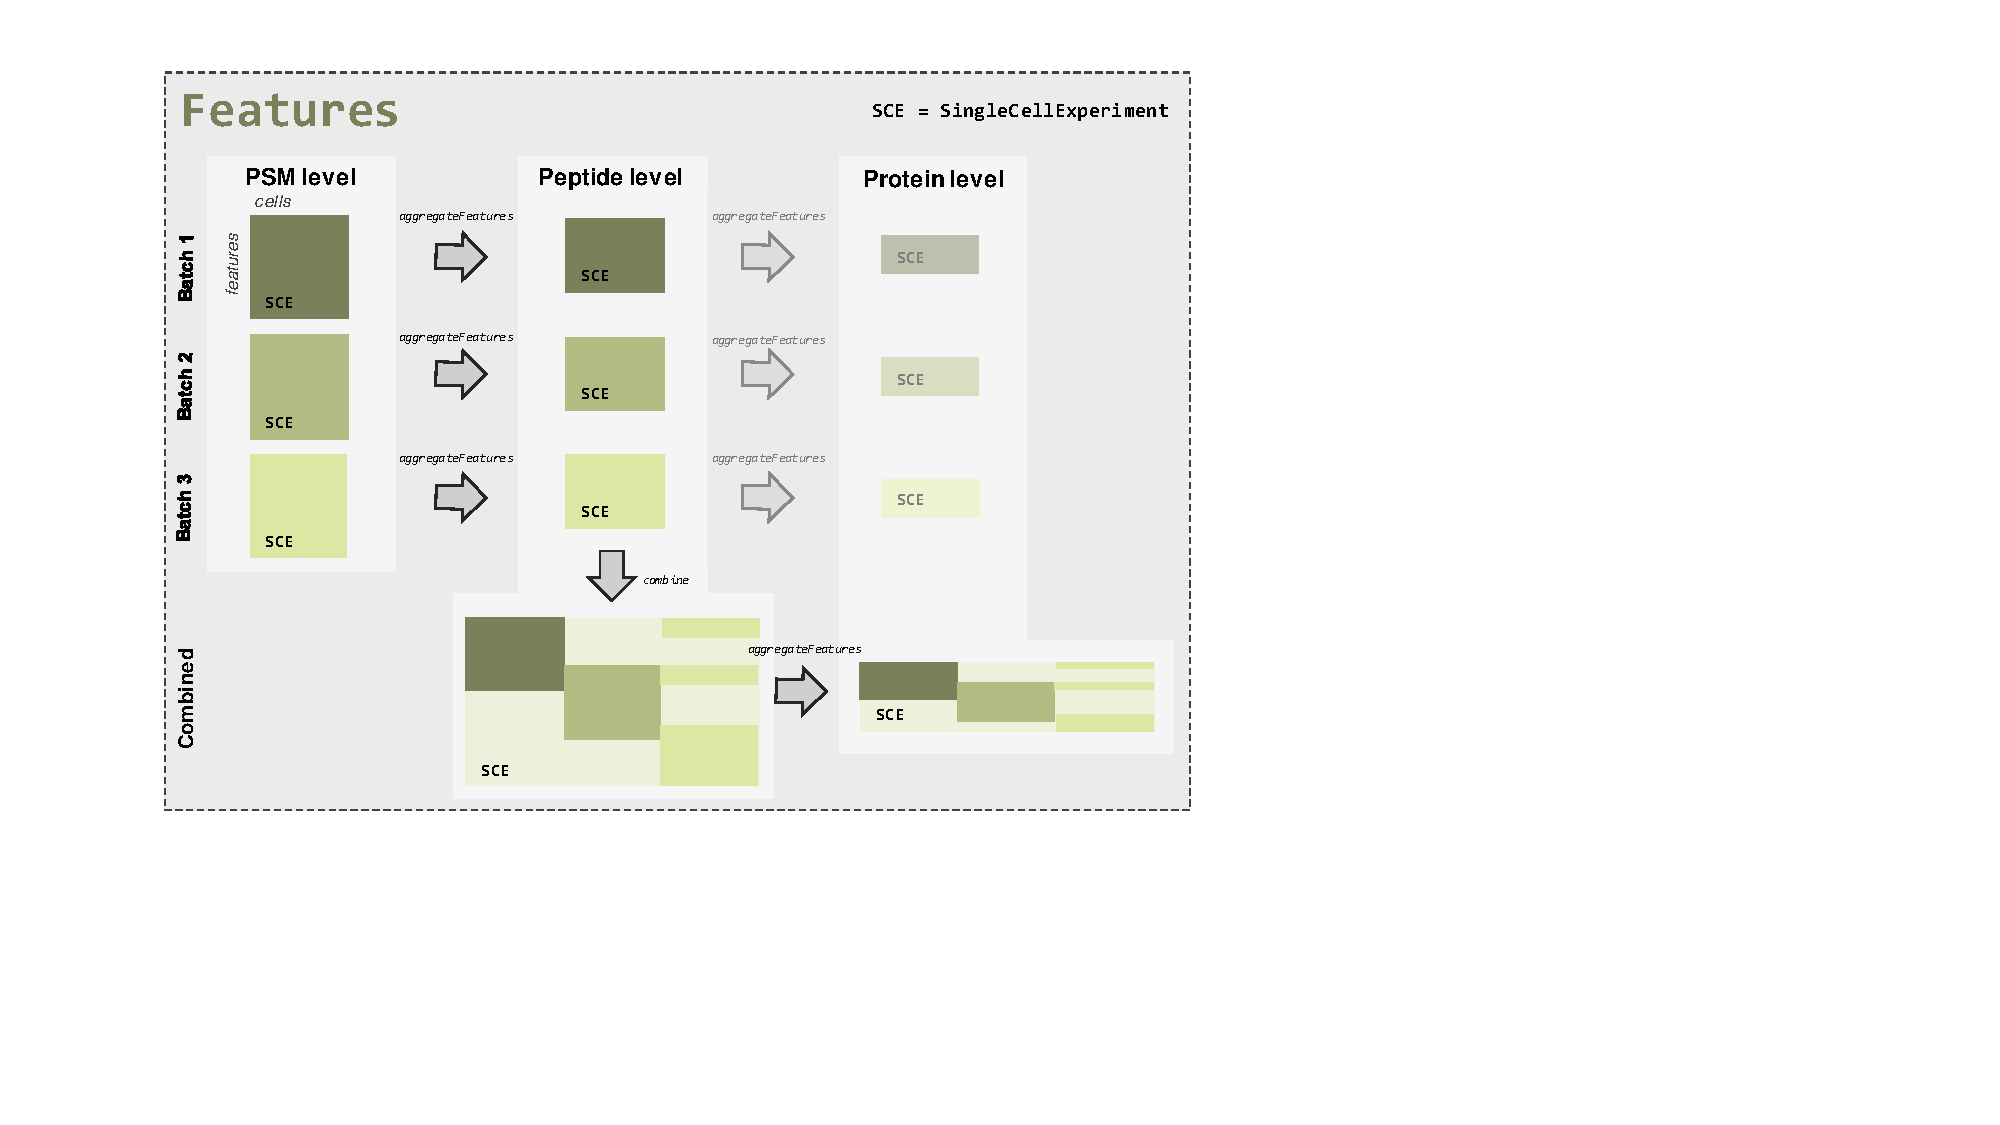
\includegraphics[width=0.9\textwidth, trim={2.6cm 5cm 14cm 1cm},clip]{figs/Features.pdf}
  \end{center}
  \hspace{3.5cm} 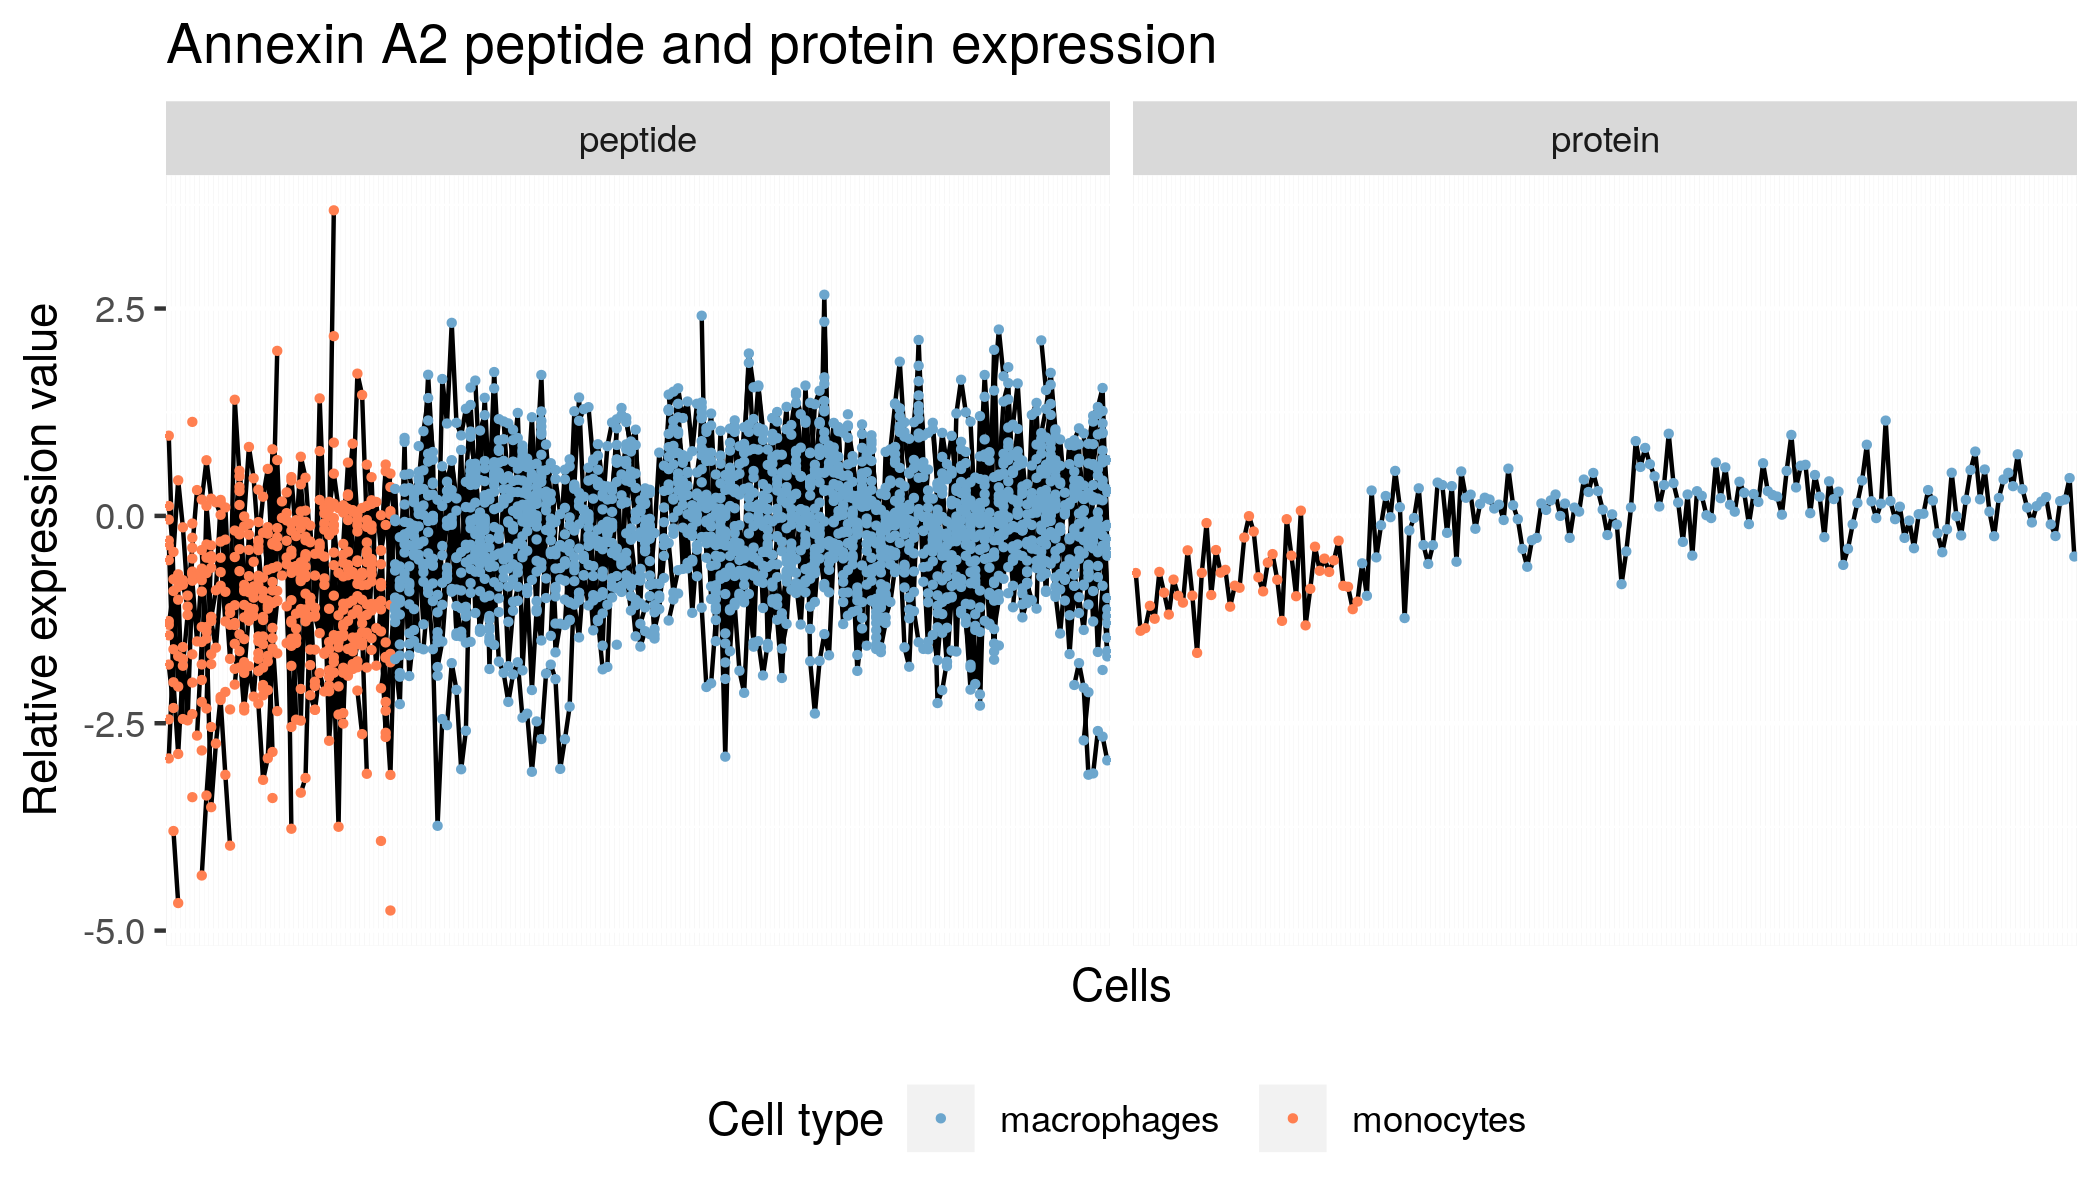
\includegraphics[width=0.7\textwidth]{figs/annexinA2.png}
\end{minipage}


% ---------------------------------------------------------------------------
% Problems to tackle
\noindent
\begin{minipage}[t]{\linewidth}
  \vspace{0.35cm}
  \section*{\huge Problems to tackle}
  \vspace{0.15cm}
\end{minipage}
  
% Batch effect
\noindent
\begin{minipage}[h]{0.5 \linewidth}
  \subsection*{Batch effects}
  \large
  Batch effects are inherent to MS-SCP data since many samples/cells have to be distributed across \textbf{different MS runs}. This leads to major biases in the data (Figure \ref{fig:pca}).
% Missingness
  \subsection*{Missingness}
\end{minipage}
\hspace{0.4cm}
% Missingness figure
\begin{minipage}[h]{0.5\linewidth}
  \begin{center}
  
\includegraphics[width=0.4\linewidth, trim={10cm 3cm 7cm 0},clip]{figs/missing-leg.png}
  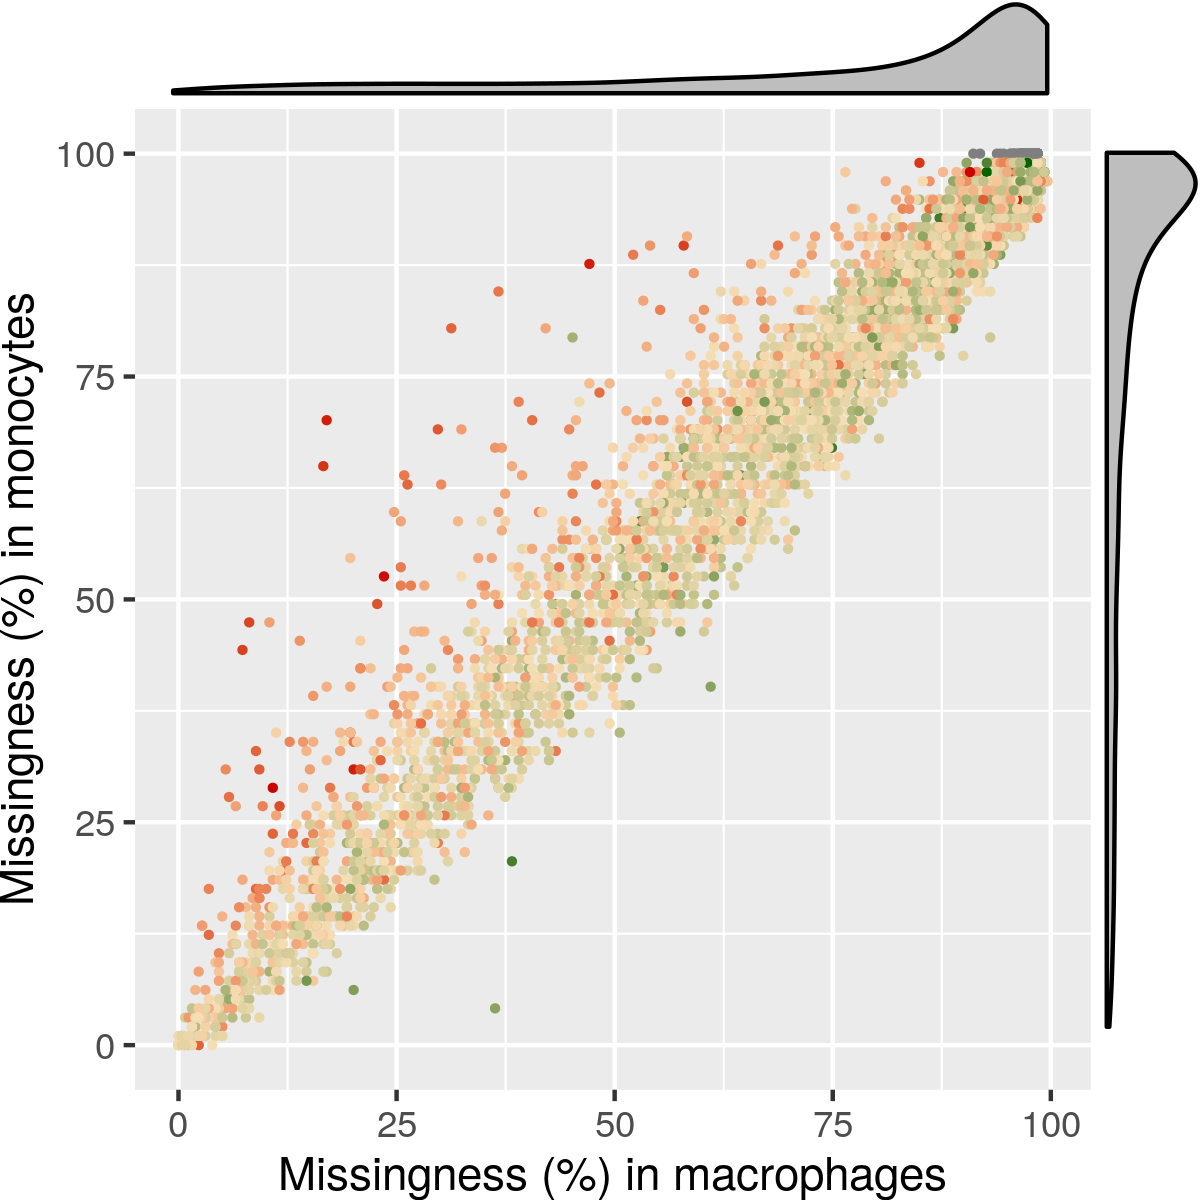
\includegraphics[width=0.8\linewidth, trim={0 2cm 0 2cm}]{figs/missing.png}
  \end{center}
\end{minipage}

% Curse of dimensionality
\noindent
\begin{minipage}[h]{\linewidth}
  \subsection*{Curse of dimensionality}
  \large
  Although current acquisition pipelines produce data sets of \textbf{thousands of peptides x hundreds of cells}, it is expected that new technological advances might raise the dimensionality 100 fold \cite{Specht2019-jm}. This is a challenge for the \textbf{statistical analyses} and for the \textbf{software optimization}. Possible solutions should be inspired from current achievements in single cell transcriptomics. 
\end{minipage}

% ---------------------------------------------------------------------------
% Additional notes
\vspace{0.5cm}
\noindent
This work is funded by an Aspirant FRS-FNRS fellowship awarded to Christophe Vanderaa. The poster is available at {\color{blue}{https://github.com/cvanderaa/EuroBioc2019-Poster}}.



% ---------------------------------------------------------------------------
% References
\scriptsize
\bibliography{ref.bib} 
\bibliographystyle{ieeetr}

% ---------------------------------------------------------------------------
% End of poster
\end{multicols}
\end{document}